% Copyright 2004 by Till Tantau <tantau@users.sourceforge.net>.


\documentclass{beamer}
\usepackage{amsmath, amsthm, amssymb}
\usepackage{graphicx}
\usepackage{float}
\usepackage{tikz}
\usepackage{pifont}
\usepackage{color}
\usepackage[font = footnotesize]{subcaption}
%\usepackage[numbers, super, sort&compress]{natbib}
%\usepackage[backend=biber,style=ieee, maxnames=4]{biblatex}
%\usepackage[superscript, biblabel]{cite}
\usepackage[backend=bibtex, bibstyle = authoryear, citestyle=authoryear, maxnames = 4, minnames = 1]{biblatex}
\addbibresource{ref.bib}

\newcommand{\cmark}{\ding{51}}
\newcommand{\xmark}{\ding{55}}

\usetikzlibrary{shapes.geometric, arrows}

\tikzstyle{input} = [rectangle, rounded corners, minimum width = 3cm,
minimum height = 1cm, text centered, draw = black, fill = red!30]
\tikzstyle{arrow} = [thick, ->, >=stealth]

\usetheme{CambridgeUS}


\title{Automated Summarisation of Big Data using Rmarkdown}
\subtitle{Using data from the Catlin Seaview Survey - a global coral reef monitoring effort}
\author{Amy Stringer}
\institute[Global Change Institute] % (optional, but mostly needed)
{
  \inst{1}%
  University of Queensland
}
\date{UseR! July 2018}

% Add logo
\pgfdeclareimage[height=0.5cm]{university-logo}{logos}
\logo{\pgfuseimage{university-logo}}

% Delete this, if you do not want the table of contents to pop up at
% the beginning of each subsection:
\AtBeginSubsection[]
{
  \begin{frame}<beamer>{Outline}
    \tableofcontents[currentsection,currentsubsection]
  \end{frame}
}

% Let's get started
\begin{document}
    \section{Introduction}
        \begin{frame}
          \titlepage
        \end{frame}

        \begin{frame}{Outline}
          \tableofcontents
          % You might wish to add the option [pausesections]
        \end{frame}

        \begin{frame}
          \begin{block}{[Insert crowd banter]}
              find out about the audience
          \end{block}
        \end{frame}

% Section and subsections will appear in the presentation overview
% and table of contents.
    \section{Context}
        \begin{frame}{The Catlin Seaview Survey}
          \begin{columns}[T]
            \begin{column}{0.45\textwidth}
              \begin{itemize}
                \item Coral reef monitoring program
                \item Endeavouring to get a global baseline on coral cover and then monitor the state of reefs through resurvey efforts
                \item 5 regions around the world so far: Australia, the Caribbean, Southeast Asia, the Indian Ocean, The Pacific
                  \begin{itemize}
                    \item Within these 5 major regions, we have 25 survey countries
                  \end{itemize}
              \end{itemize}
            \end{column}

            \begin{column}{0.45\textwidth}
              \vskip-\baselineskip
                \begin{figure}
                  \centering
                      \begin{subfigure}[t]{0.6\textwidth}
                        \centering
                        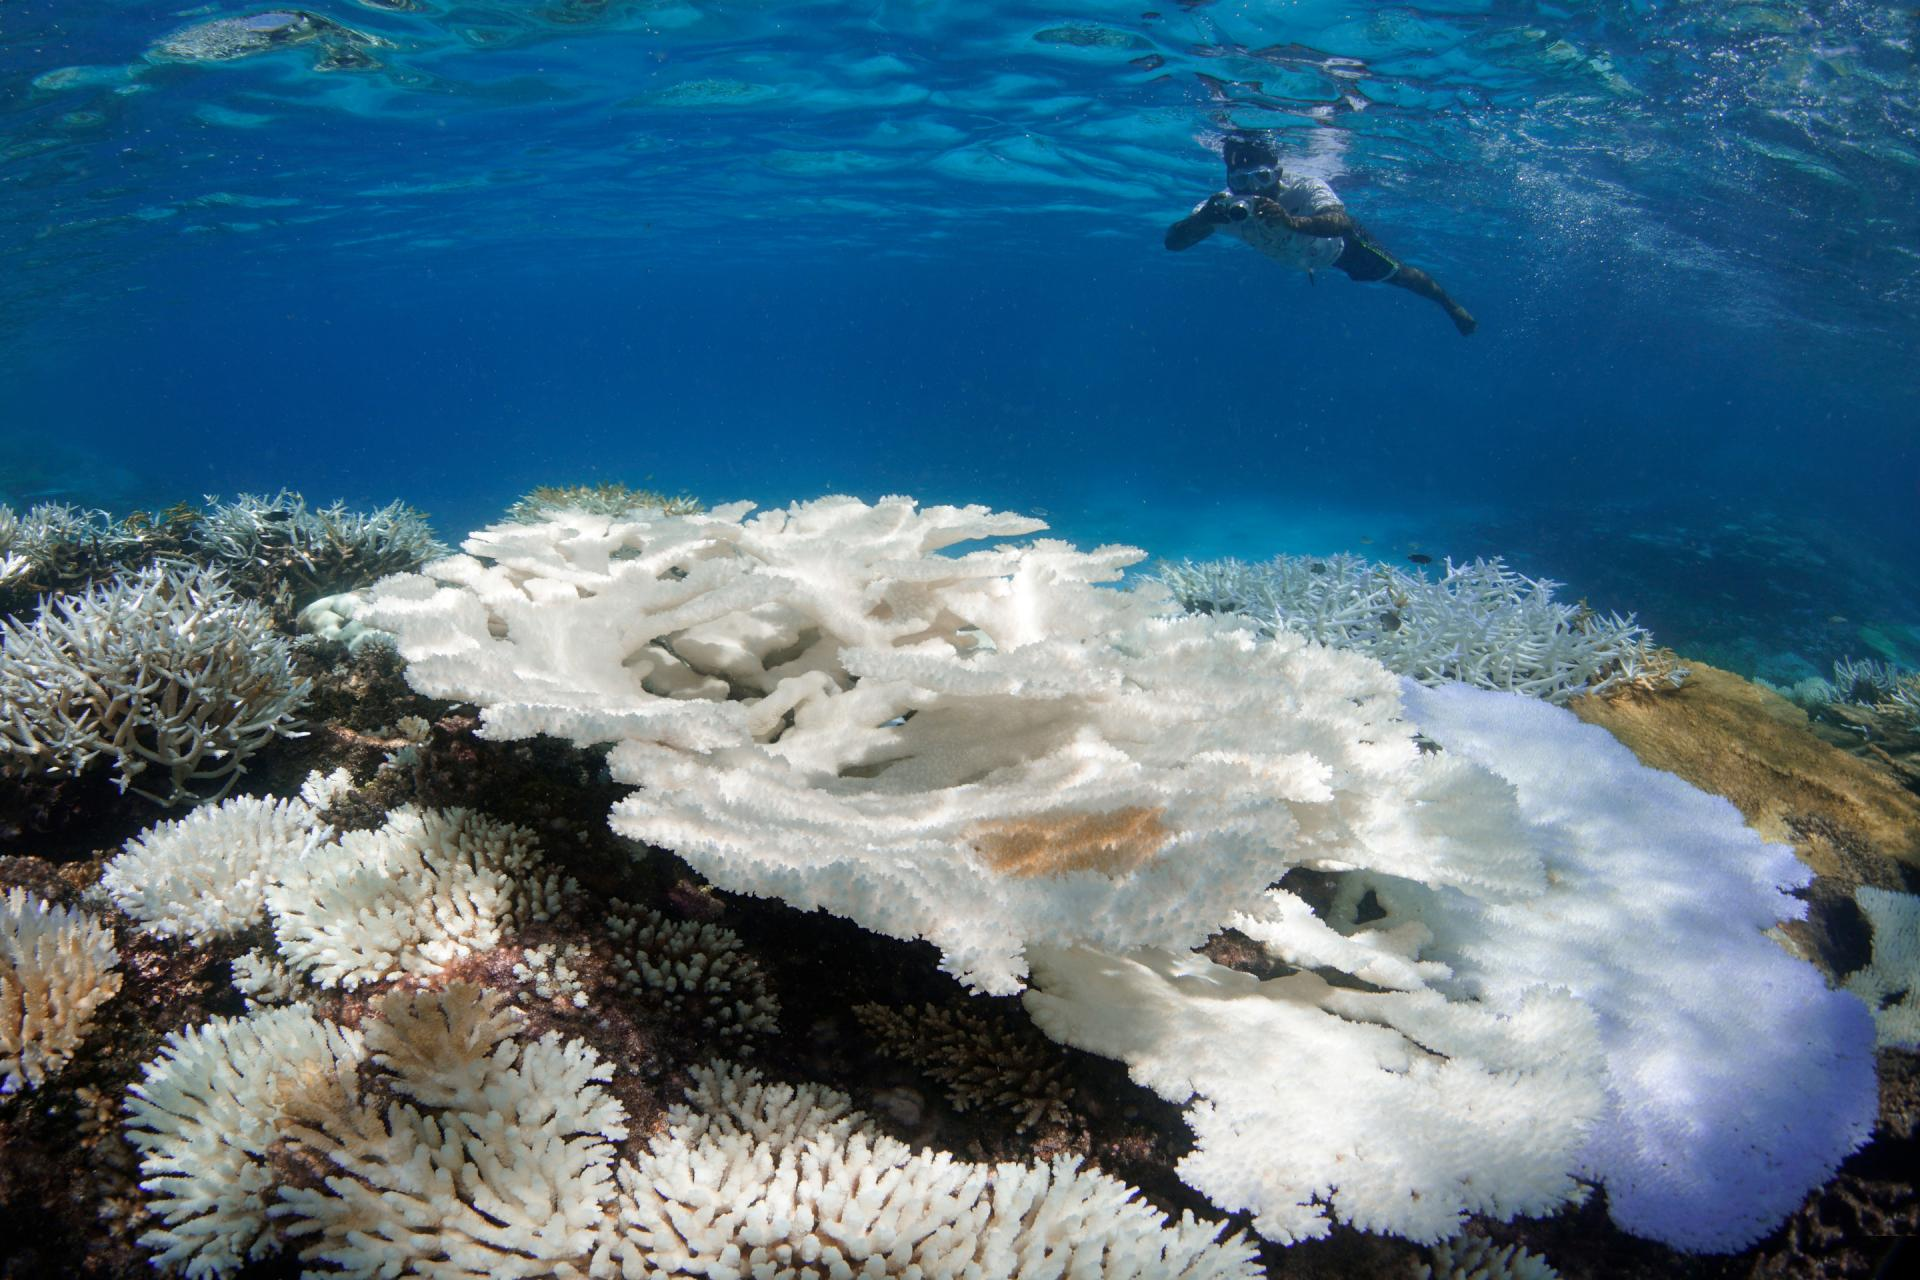
\includegraphics[width = \linewidth]{bleach1_maldives.jpeg}
                        \caption{Bleaching at the Maldives, 2016}
                        \label{fig:bleach_maldives}
                      \end{subfigure} \hskip 1em%
                      \begin{subfigure}[t]{0.6\textwidth}
                        \centering
                        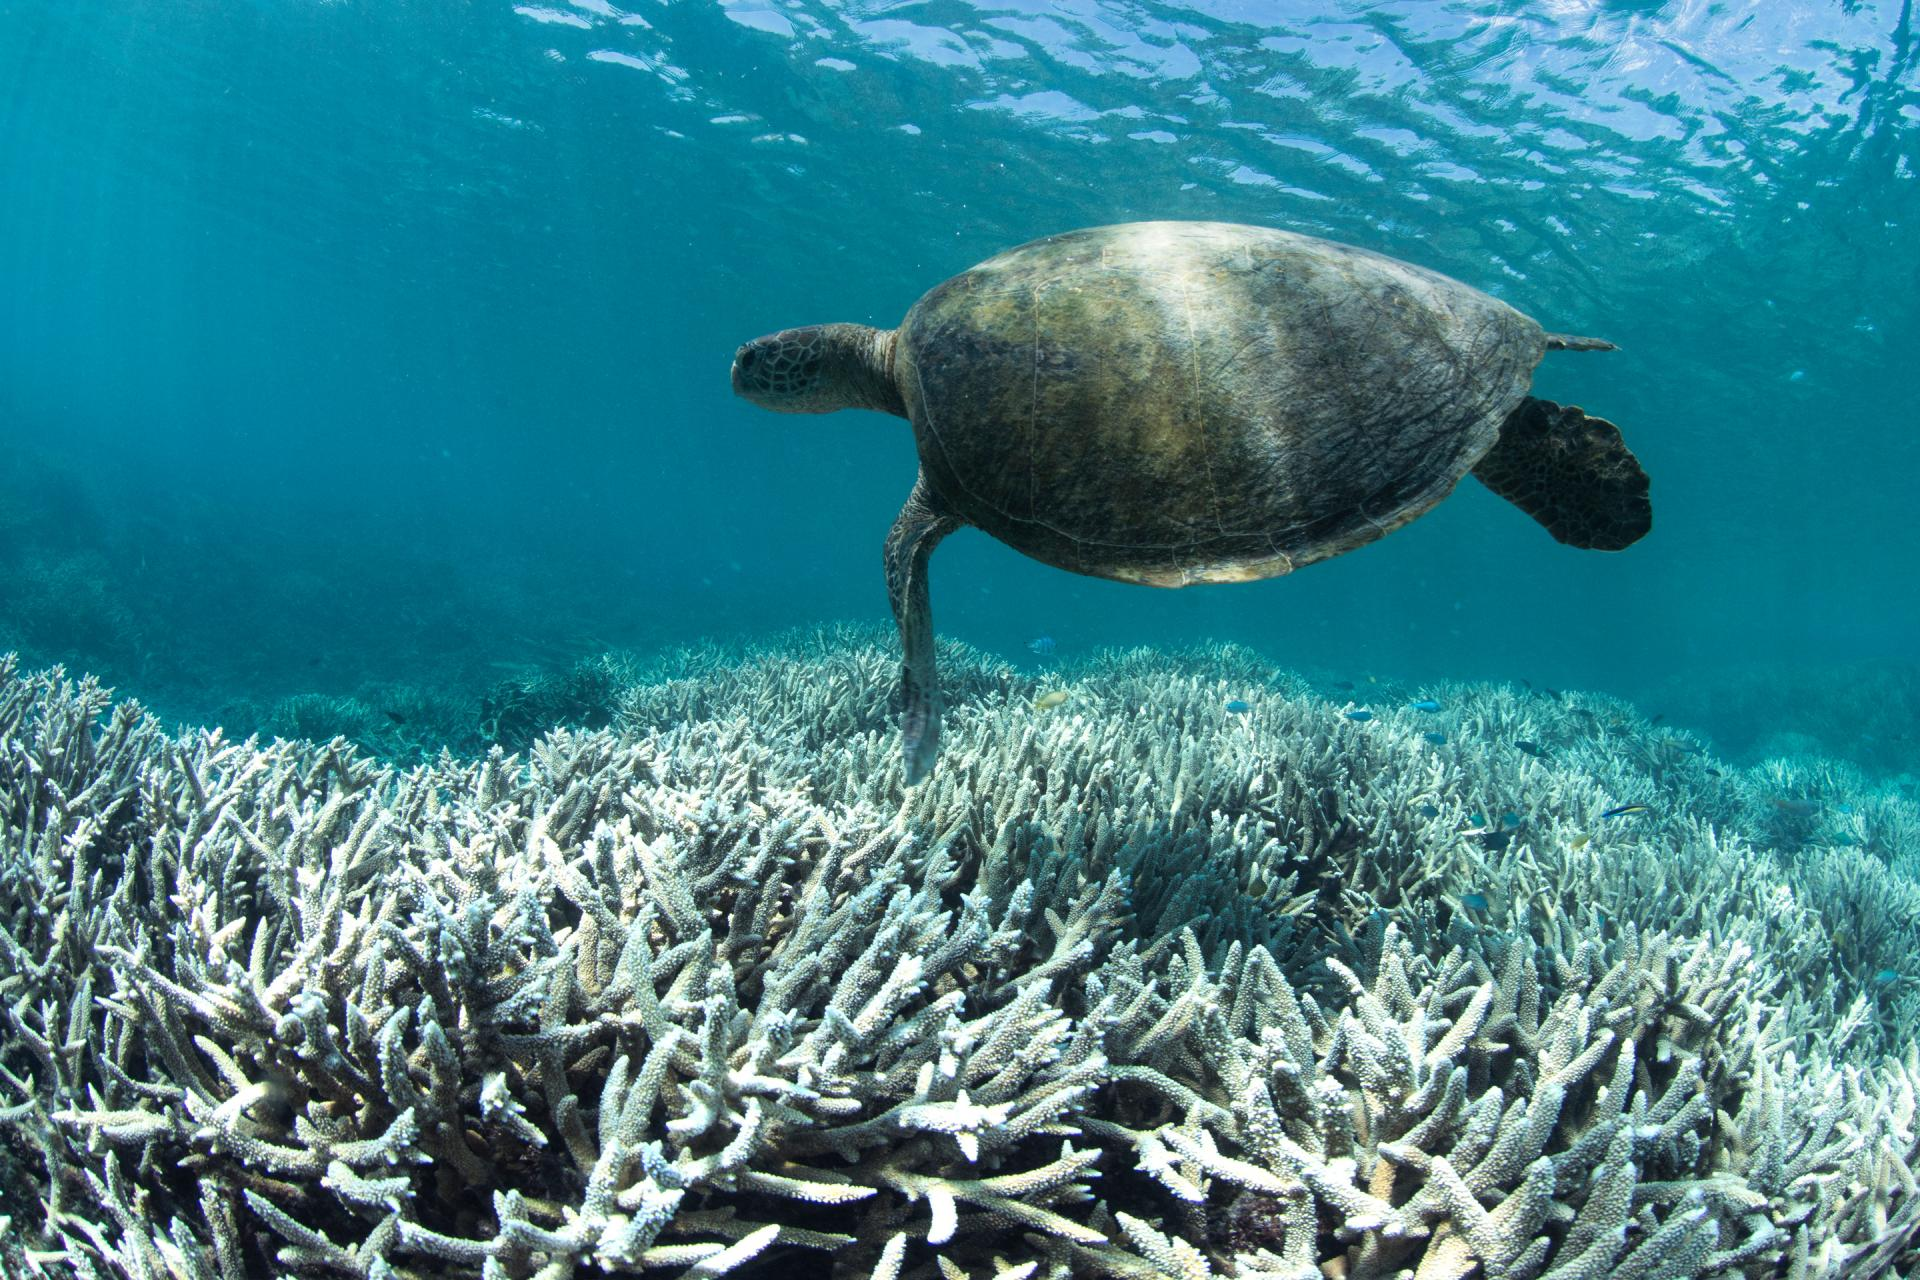
\includegraphics[width = \linewidth]{bleach3_heron.jpeg}
                        \caption{Bleaching at Heron Island, 2016}
                        \label{fig:bleach_heron}
                      \end{subfigure}
                \end{figure}
            \end{column}
          \end{columns}
        \end{frame}

        \subsection{The Catlin Data}
            \begin{frame}{Efficient Monitoring}
                Three main stages:
                  \begin{enumerate}
                    \item Collection of images
                    \item Annotation of images
                    \item Calculating proportions, and visualing trends between surveys
                  \end{enumerate}
            \end{frame}

        \subsection{Image Collection}
            \begin{frame}{The Catlin Seaview Survey - Image Collection }
                \begin{figure}
                    \centering
                    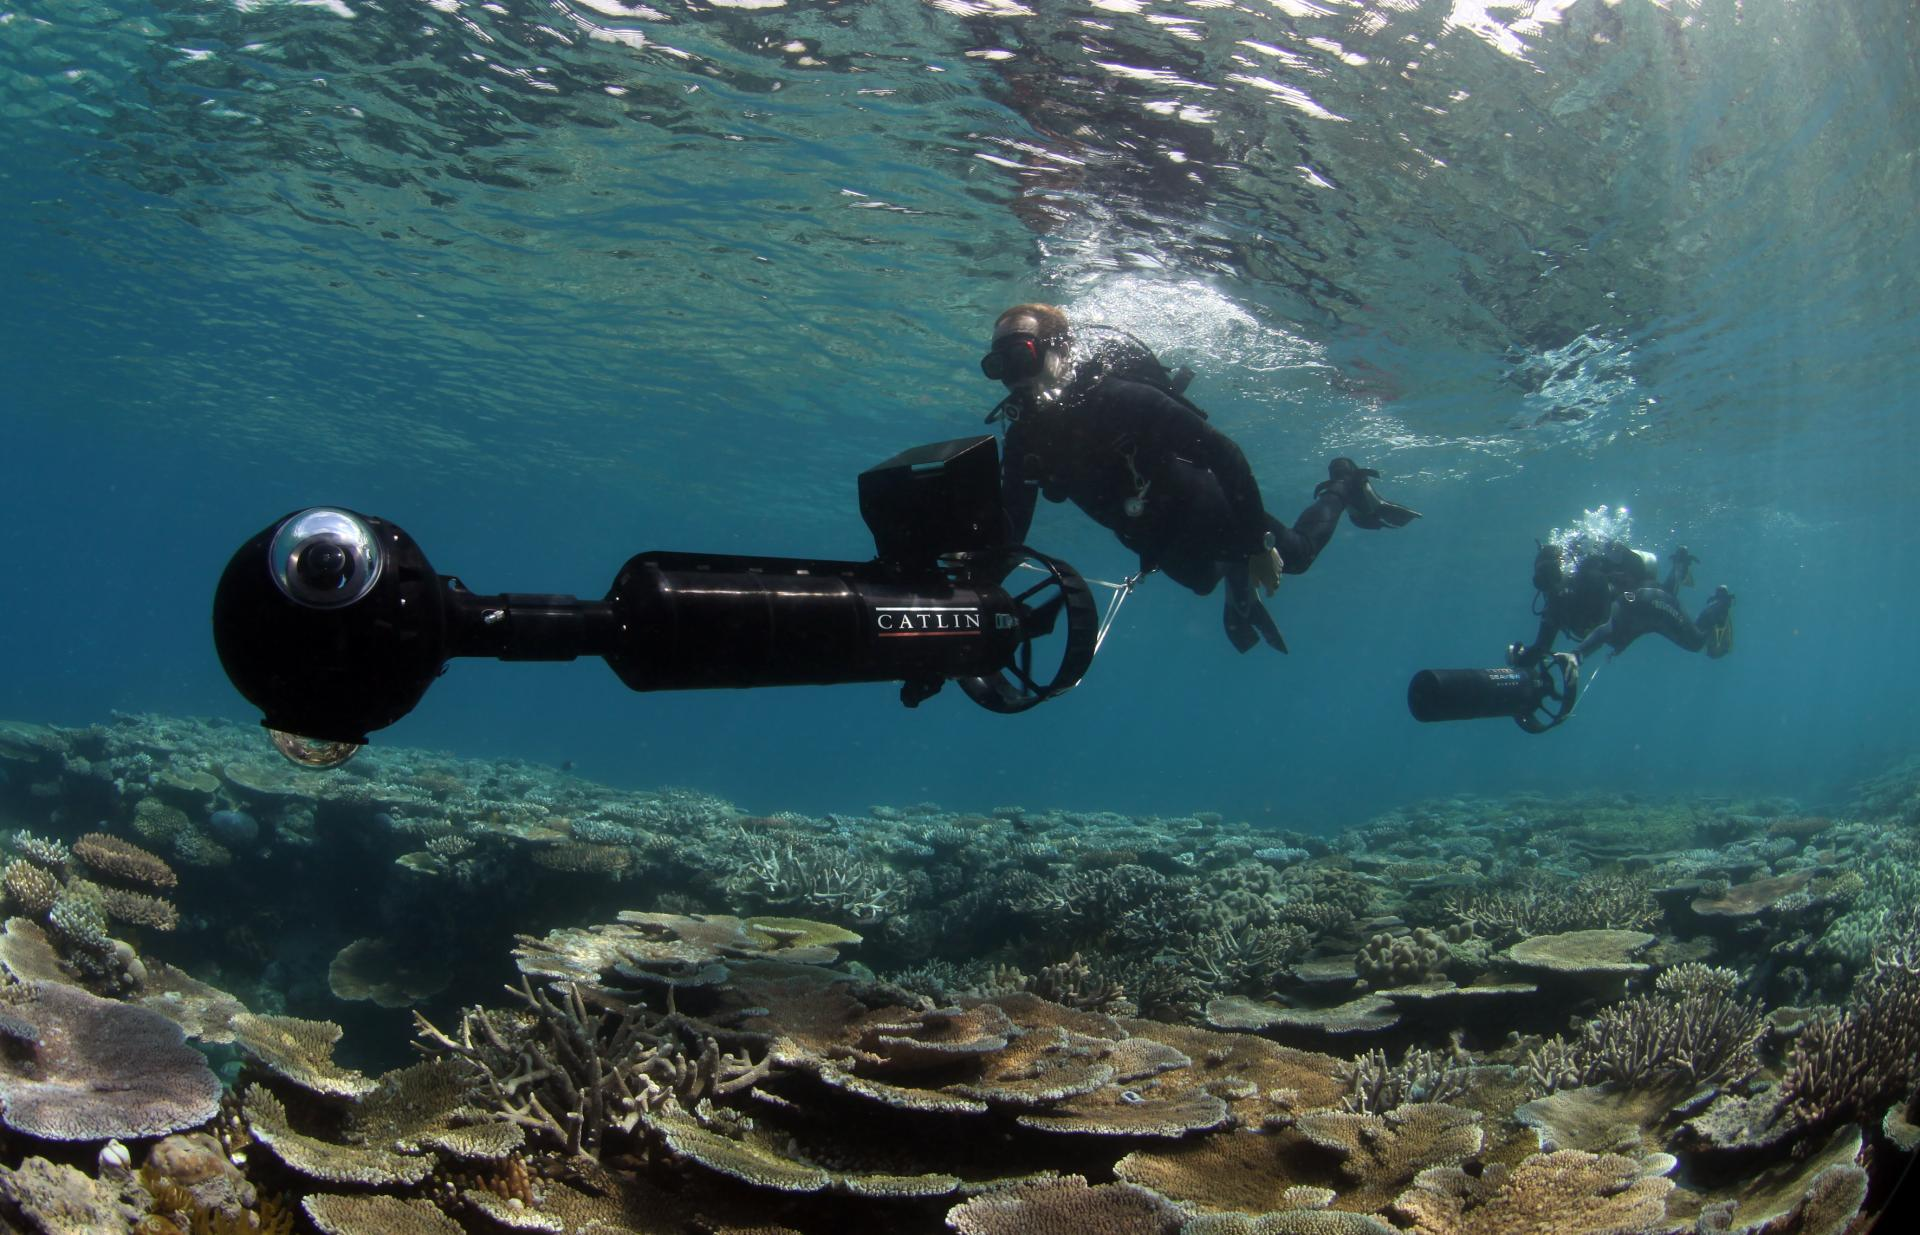
\includegraphics[width = 0.65\textwidth]{SVII.jpg}
                    \caption{{\footnotesize A diver pushing the SVII scooter during a survey of the Great Barrier reef, for more on collection methodology, see \cite{Gonz16} \copyright XL Catlin Seaview Survey}}
                \end{figure}
            \end{frame}

            \begin{frame}{Notes}
                \begin{itemize}
                  \item Images collected in 2km transects along a reef \cite{Gonz14}
                  \item An image taken automatically every three seconds as a diver swims along the reef section
                  \item Each image is GPS located
                  \item speed of image collection compared to traditional methods
                \end{itemize}
            \end{frame}

            \begin{frame}
                \begin{figure}
                    \centering
                    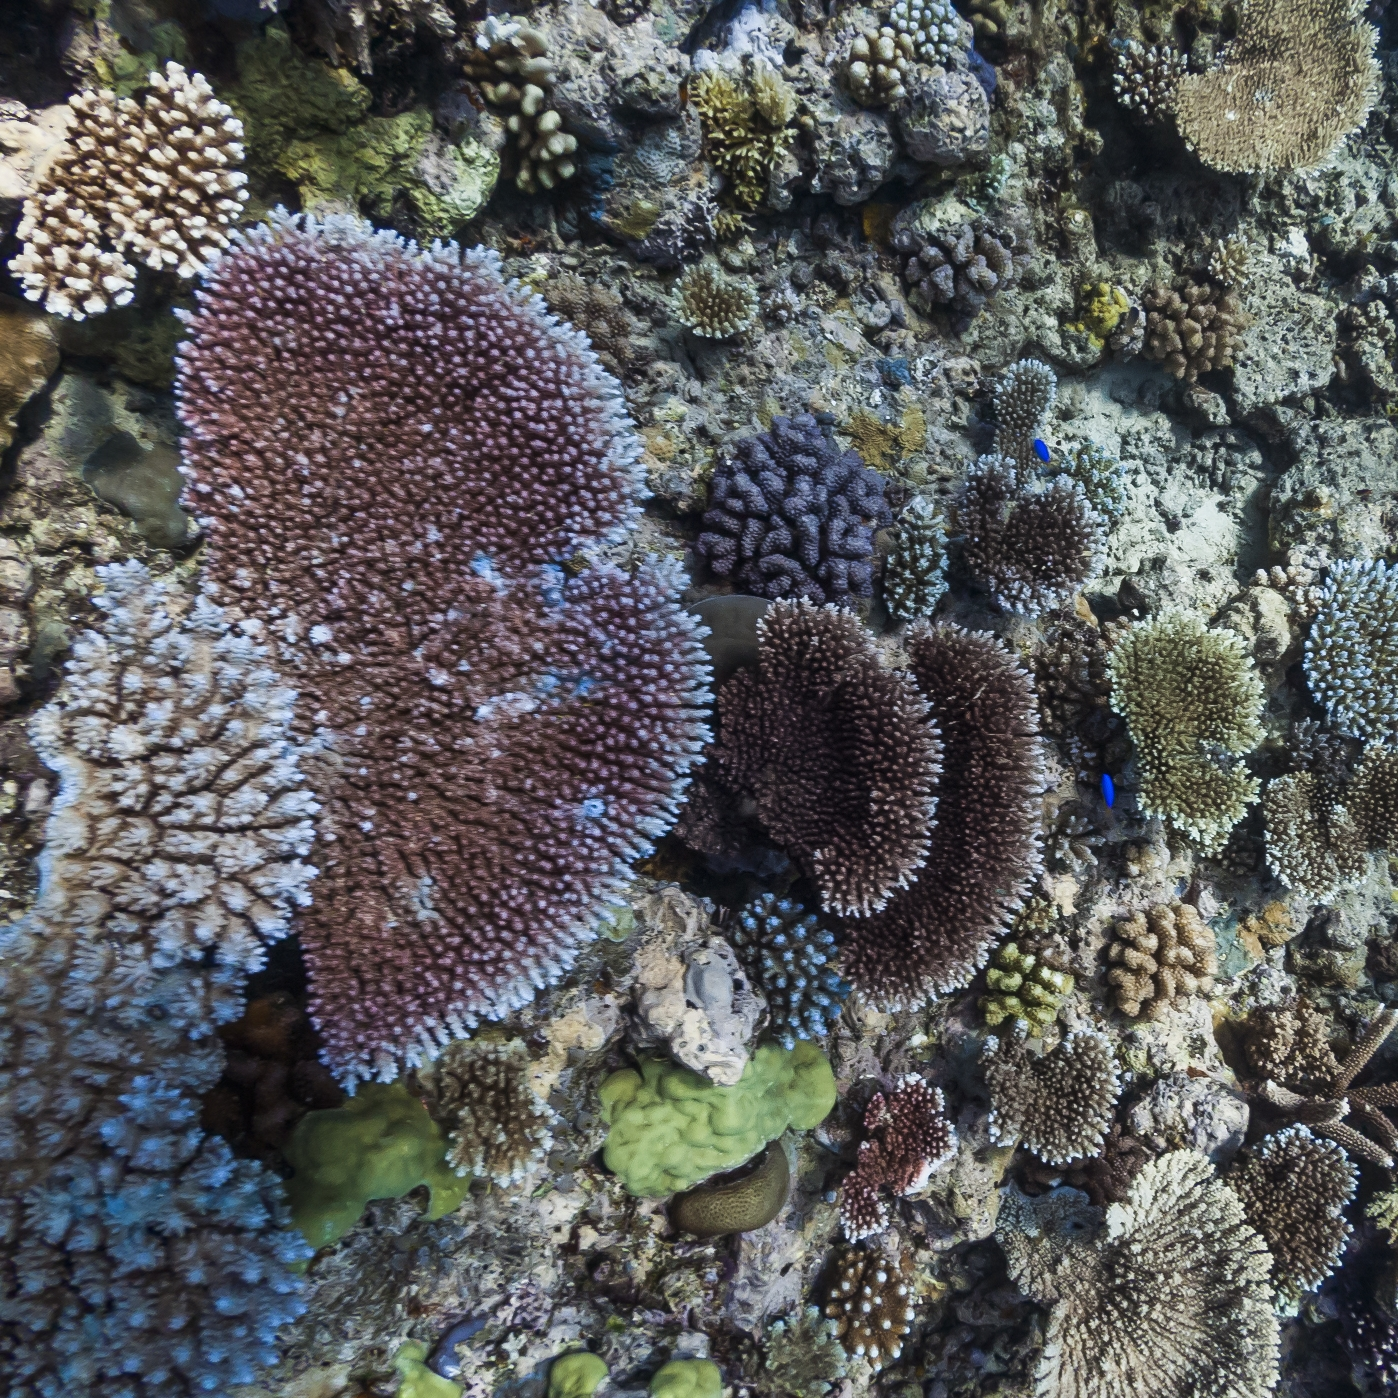
\includegraphics[width = 0.5\textwidth]{coral.jpg}
                    \caption{An example image from a survey of the Great Barrier Reef}
                \end{figure}
            \end{frame}

          \subsection{Image Annotation}
              \begin{frame}{Neural Network for Image Annotations}
                  Using a neural network means that the image annotation process is efficient, with data being uploaded to the database only a week after collection of images is concluded
              \end{frame}

              \begin{frame}
                  \begin{figure}
                      \centering
                      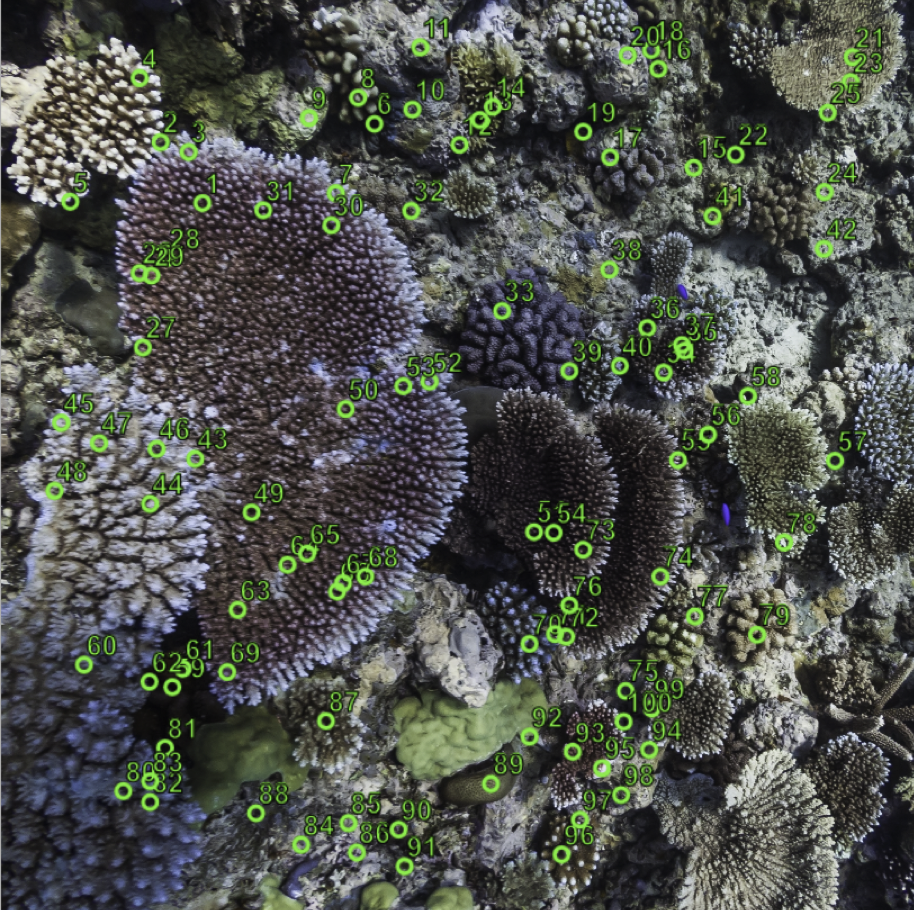
\includegraphics[width = 0.5\textwidth]{coral_points.jpg}
                      \caption{The same image from earlier showing the points used for annotation}
                  \end{figure}
              \end{frame}

              \begin{frame}{Revisting}
                  Three main stages:
                    \begin{enumerate}
                      \item <1->{
                      Efficient collection of images \uncover<2->{ \cmark}
                      }
                      \item <3-> {
                      Efficient annotation of images \uncover<4-> { \cmark}
                      }
                      \item <5-> {
                      Efficient calculation proportions, and visualisation of trends over all regions \uncover <6-> { \xmark}
                      }
                    \end{enumerate}
              \end{frame}

    \section{The Need}
        \subsection{Efficient Summarisation}
            \begin{frame}{The Next Stage}
                \begin{itemize}
                  \item there's now a ``bottleneck'' in the analysis process
                  \item fast data collection $\rightarrow$ fast annotation $\rightarrow$ slow to process
                  \item The third stage was lacking an efficient process
                  \item annotation output stored in a MySQL database, allows for easy integration with R
                  \item Introducing Rmarkdown (\cite{rmarkdown})
                  \item rmarkdown provides a solution for quick/consistent exploratory analysis of the data
                \end{itemize}
            \end{frame}


      \section{New Challenges}

        \subsection{Contextual Challenges}
            \begin{frame}{Contextual Challenges}
                \begin{itemize}
                    \item Meaningful visualisations for those who will be using them
                    \begin{itemize}
                       \item these reports need to be useful for more than just the researchers, decision makers need to get some value out of them too
                    \end{itemize}
                    \item Usability for non R users
                    \begin{itemize}
                      \item this will allow me to talk about the use of parameters on the document and the use of child documents for textual portions of the reports
                    \end{itemize}
                \end{itemize}
              \end{frame}

        \subsection{Data Challenges}
            \begin{frame}{Data Challenges - Structure}
                \begin{center}
                  \begin{table}
                    \begin{tabular}{l r r r}
                      Sub-region            &   Reef Count      &   Transect Count      &   Image Count           \\ \hline
                      Cairns-Cooktown       &   13              &   43                  &   87631                 \\
                      Coral Sea             &   3               &   32                  &   23573                 \\
                      Far Northern          &   12              &   33                  &   68367                 \\
                      Mackay-Capricorn      &   4               &   12                  &   14151                 \\
                      Townsville-Whitsunday &   4               &   10                  &   5722                  \\
                      Total                 &   36              &   130                 &   {\color{red}{199444}} \\
                    \end{tabular}
                      \label{tab:GBRSummary}
                      \caption{A summary of the various spatial scales within just one region, the Great Barrier Reef. This structure is consistent across all 5 regions.}
                  \end{table}
                \end{center}
            \end{frame}

            \begin{frame}{Data Challenges - Labels}
                \begin{itemize}
                  \item talk about the label set and need to visualise changes at all of these levels (label, global label and functional group)
                \end{itemize}
            \end{frame}

      \section{Solutions}
          \subsection{RMySQL and Parameterised Rmarkdown}
              \begin{frame}{RMySQL}
                  \begin{itemize}
                    \item allows for accessing the database through Rstudio
                  \end{itemize}
              \end{frame}

              \begin{frame}{Parameterising Rmarkdown Documents}
                        \begin{figure}
                          \centering
                          \begin{subfigure}[t]{0.48\textwidth}
                            \centering
                              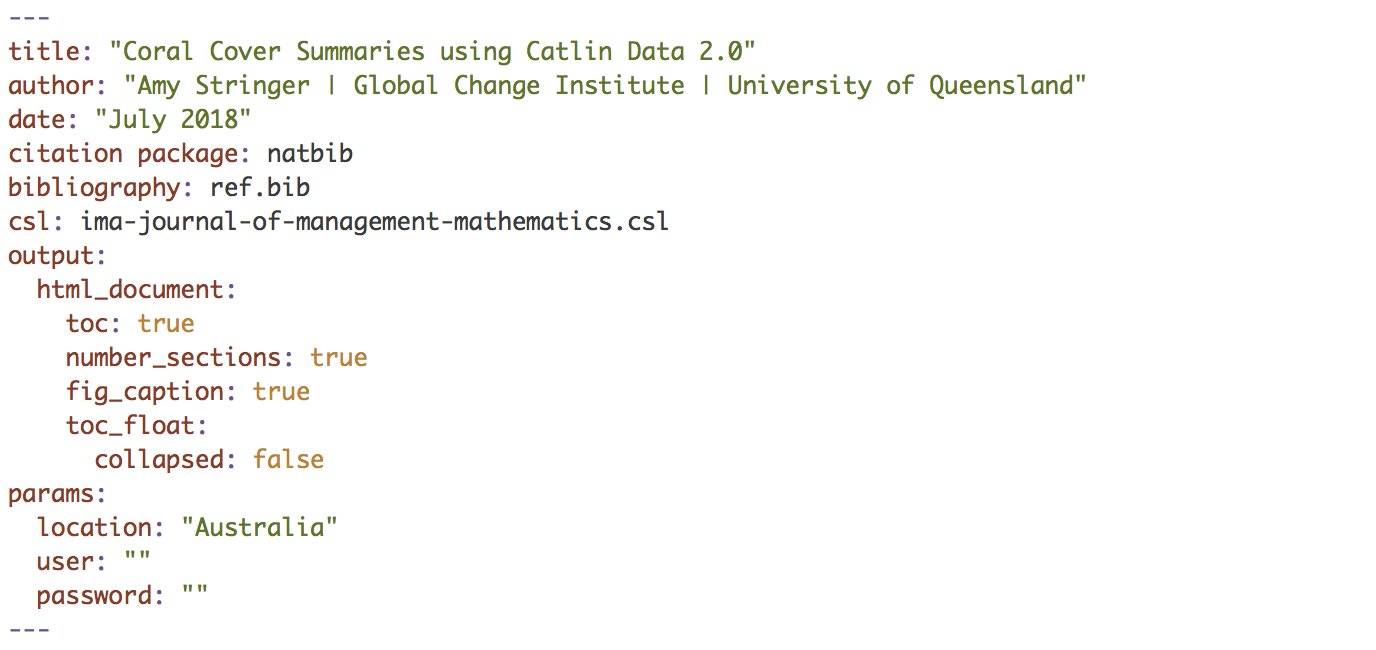
\includegraphics[width = \textwidth]{yaml_header.png}
                              \caption{yaml header when making use of document parameters}
                              \label{fig:yaml_header}
                          \end{subfigure}\hskip 1em%
                          \begin{subfigure}[t]{0.48\textwidth}
                            \centering
                              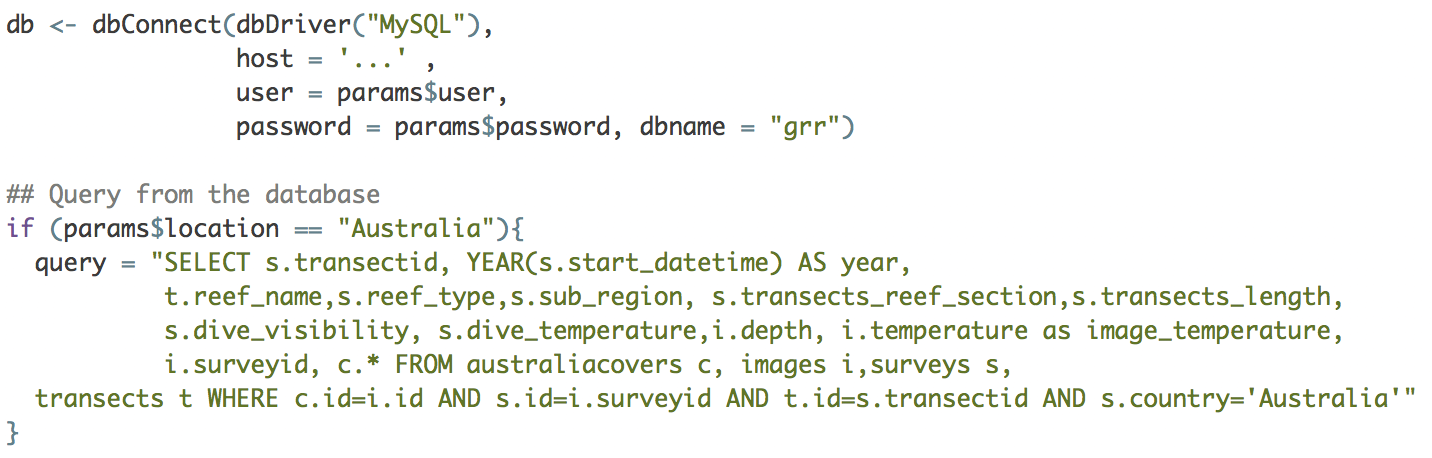
\includegraphics[width = \textwidth]{SQL_connect.png}
                              \caption{Working example accessing the database with the document input parameters}
                              \label{fig:SQL_connect}
                          \end{subfigure}
                        \end{figure}
                \end{frame}

                \begin{frame}{Notes}
                    \begin{itemize}
                      \item added parameters for location, as well as user and password for the databse
                      \item allows us to select a location through the use of render()
                      \item this also allows users to add in their username and password for database access
                    \end{itemize}
                \end{frame}

          \subsection{Child Documents}
              \begin{frame}{Child Documents for Textual Components}
                  \begin{itemize}
                    \item Introductions and discussions will need to be different across the regions
                    \item Using the parameters of the documents we can include a particular introduction file for each specific region
                    \item This also allows for easy editing should that be necessary, without needing to open the main rmardown document which could be overwhelming and complicated for those the reports are designed for
                  \end{itemize}
              \end{frame}

          \subsection{Dynamic Plotting Environments}
              \begin{frame}{Dynamic Plotting }
                  \begin{itemize}
                    \item different regions have a different labelset, which makes visualisation a different challenge for each subset of the data
                    \item the code wrapper in the rmarkdown source script allows you to set a variable to the figure heights and widths
                    \item many regions have only one survey and so many of the plots break without some kind of conditioning on their construction
                  \end{itemize}
              \end{frame}

          \subsection{Interactive Maps using Leaflet}
              \begin{frame}{Leaflet}
                  \begin{itemize}
                    \item Handy for readers to see where exactly the surveys take place
                    \item Ideally this marker would be a measure from the center of each transect or reef, but the marker point is taken to be the GPS coords of the first image in a transect/reef
                    \item At this stage the maps only show reef name and transect number which appeals to perhaps local monitoring teams (Reef scale) and the survey/image collection teams (transect number)
                  \end{itemize}
              \end{frame}








% All of the following is optional and typically not needed.
\appendix
\section<presentation>*{\appendixname}
\subsection<presentation>*{For Further Reading}

\begin{frame}[allowframebreaks]
  \frametitle<presentation>{References}
    %\bibliographystyle{agsm}
    \printbibliography
  \end{frame}

\end{document}
